\section{Branching ratio of top quark decay}
\label{s:brThb}
Being a very short-lived particle with a lifetime of $5\times 10^{-25}$\unit{s}, the
\PQt quark decays immediately. In the SM, it decays only to W boson
and \PQb quark as its decay involving other quarks (s, d) is suppressed
by the corresponding element of the CKM matrix. The ratio R = \brTwb/\brTwq 
where q = \PQb, \PQs, and \PQd is 0.90 $\pm$ 0.04 as was earlier 
determined from D0 experiment using 5.4 $\fbinv$ 
data \cite{PhysRevLett.107.121802}. The CDF experiment using 162 
pb$^{-1}$ luminosity has put a lower bound at 95\% CL on it, 
R $>$ 0.61 \cite{PhysRevLett.95.102002}. The latest lower bound, R $>$ 
0.95, is obtained from the CMS experiment at 8 \TeV using 19.7\fbinv 
luminosity \cite{Khachatryan:2014nda}  which suggests that the \PQt 
quark can have other decay channels beyond the SM. In the 2HDM, it is allowed to 
decay into $H^+q$ channel. The branching ratio of this decay process is given by
\begin{equation}
BR(t\to H^+q) = \frac{\Gamma(t\to H^+q)}{\Gamma(t\to W^+q)+\Gamma(t\to H^+q)}
\label{eq:brThb}
\end{equation}
where $\Gamma(t\to H^+q)$ and $\Gamma(t\to W^+q)$ are the partial decay widths. 
For the \PQb quark, these decay widths are given as \cite{PhysRevD.80.015017}
\begin{align}
\Gamma(t\to H^+b) =&
\frac{G_F\left|V_{tb}\right|^2}{8\sqrt2\pi m_t}
\lambda\left(\frac{m_b^2}{m_t^2},\frac{m_{H^\pm}^2}{m_t^2}\right)^{1/2}
\nonumber\\
&\times
\left\{m_t^2\left[m_t^2{G_A^u}^2\left(1+\frac{m_b^2}{m_t^2}-\frac{m_{H^\pm}^2}{m_t^2}\right)+m_b^2{G_A^d}^2\right]
+4m_t^2m_b^2G_A^uG_A^d\right\},
\end{align}
and 
\begin{equation}
\Gamma(t\to W^+b) = \frac{G_F\left|V_{tb}\right|^2}{8\sqrt2\pi}m_t^3
\end{equation}
where
\begin{equation}
\lambda(x,y) = 1+x^2+y^2-2x-2y-2xy,
\end{equation}
and \mt = 166 \GeV (running mass of the \PQt quark), $m_b$ (running mass of \PQb quark) = 3.0 \GeV, $G_{F}$ = 
$1.1663\times 10^{-5}$, and $V_{tb}$ = 0.99. The variation of \brThb as 
a function of $\tan\beta$ and the mass of the charged Higgs is shown in Figure~\ref{fig:brThb}. 
From the plots shown on the left side, it can be seen that for low $\tan\beta < 1$, the $\brThb$ is 
the same for all the types 
of 2HDM. For higher $\tan\beta$, the \brThb increases in the Type II model as compared to Type X.
The similar $\tan\beta$ dependence can be explicitly seen from the right hand plots of this figure. Note that \brThb is the same for Type I and X, and for Type II and Y as the coupling 
of quarks with charged Higgs is same as shown in Table~\ref{tab:coupling2HDM}. 
We also see that \brThb does not change much with respect to the mass of charged Higgs
for \mHp $<$ 150 \GeV.

\begin{figure}
\centering  
\subfigure[]
	{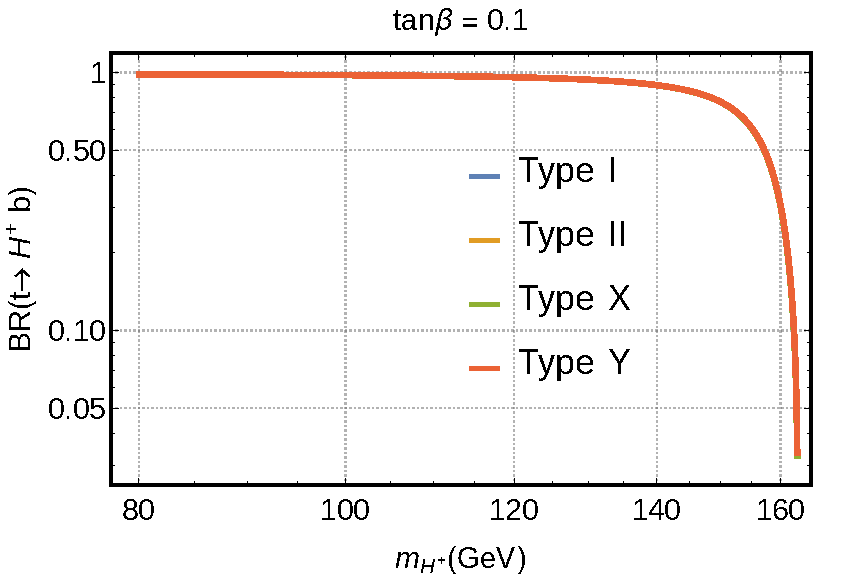
\includegraphics[width=0.45\linewidth]{Theory/Image/BR_topToHb_b0p1.pdf}}
\subfigure[]
	{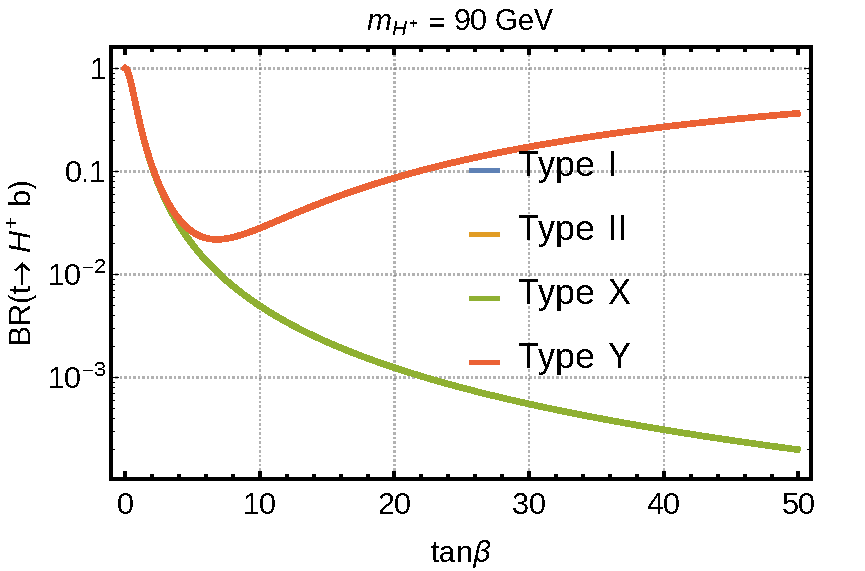
\includegraphics[width=0.45\linewidth]{Theory/Image/BR_topToHb_mH90.pdf}}
\vfil
\subfigure[]
	{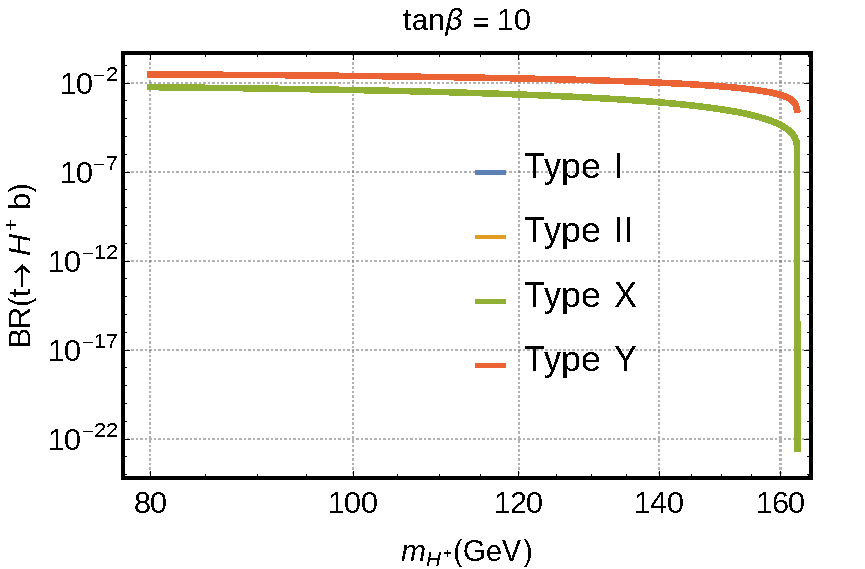
\includegraphics[width=0.45\linewidth]{Theory/Image/BR_topToHb_b10.pdf}}
\subfigure[]
	{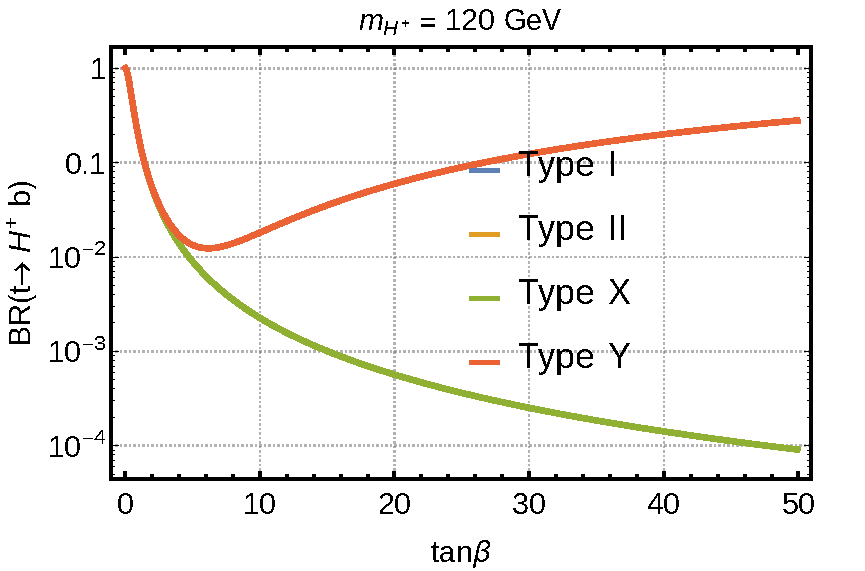
\includegraphics[width=0.45\linewidth]{Theory/Image/BR_topToHb_mH120.pdf}}
\vfil
\subfigure[]
	{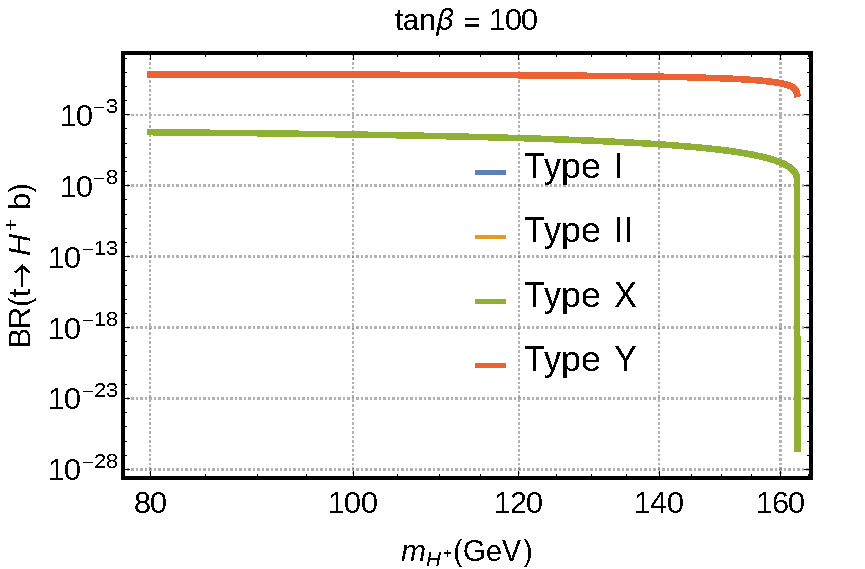
\includegraphics[width=0.45\linewidth]{Theory/Image/BR_topToHb_b100.pdf}}
\subfigure[]
	{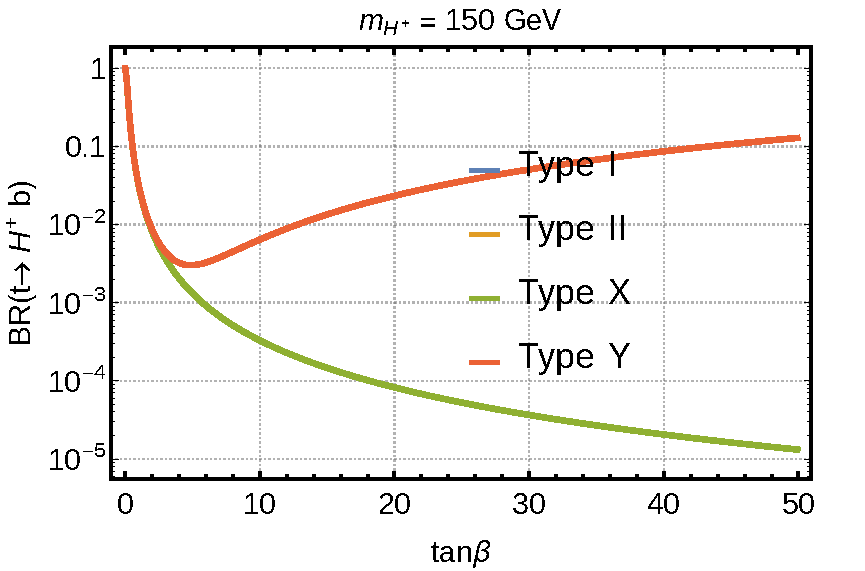
\includegraphics[width=0.45\linewidth]{Theory/Image/BR_topToHb_mH150.pdf}}
\caption{Variation of \brThb as a function of the mass of the charged Higgs 
	(left side plots) and $\tan\beta$ (right side plots).}
\label{fig:brThb}
\end{figure}

\section{Branching ratio of charged Higgs decay}
\label{s:brHqq}
For the search of charged Higgs boson, it is very important to study all of its 
possible decay channels to have an estimate of the dominance of respective
channels for a given value of $\tan\beta$, \mHp, etc. In the 2HDM, the charged
Higgs is allowed to decay into fermions and gauge bosons, for example, 
$H^+ \rightarrow c\bar{s}$, $H^+ \rightarrow c\bar{b}$, 
$H^+ \rightarrow t\bar{b}$, $H^+ \rightarrow \tau^+\nu_\tau$, 
$H^+ \rightarrow W^+\gamma$, $H^+ \rightarrow W^+Z$, $H^+ \rightarrow hW^+$, 
$H^+ \rightarrow HW^+$, and $H^+ \rightarrow AW^+$. The partial decay width of charged 
Higgs decaying to quarks and leptons is given by \cite{PhysRevD.80.015017}
\begin{align}
\Gamma(H^+\to u{\bar d}) = N_C
\frac{G_Fm_{H^\pm}^{}\left|V_{ud}\right|^2}{4\sqrt2\pi}\beta_{ud}^{}
\left\{\left(m_u^2{G^u_A}^2+m_d^2{G^d_A}^2\right)
\left(1-\frac{m_u^2+m_d^2}{m_{H^\pm}^2}\right)-\frac{4m_u^2m_d^2
{G^u_A}{G^d_A}}{m_{H^\pm}^2}\right\},
\label{Eq:H+ud}
\end{align}
and 
\begin{align}
\Gamma(H^+\to \ell^+\nu) =
\frac{G_Fm_{H^\pm}^{}m_\ell^2}{4\sqrt2\pi}{G^\ell_A}^2
\left(1-\frac{m_\ell^2}{m_{H^\pm}^2}\right)^2
\label{Eq:H+nul}
\end{align}
where 
\begin{align}
\beta_{XY}^{} &= \lambda^{1/2}\left(\frac{m_X^2}{m_\varphi^2},
\frac{m_Y^2}{m_\varphi^2}\right),
\end{align}
and $ N_C = 3, ~V_{cs} = 0.97, ~m_c = 0.81$\GeV, $m_s = 0.046$ \GeV, $V_{cb} = 
0.0412, ~m_\tau = 1.77$ \GeV, $m_\mu = 0.105$ \GeV. The total decay width of charged
Higgs decaying into fermions is given by
\begin{align}
\Gamma(H^+\to \rm{All}) = \Gamma(H^+\to \tau^+\nu) + \Gamma(H^+\to c\bar{s}) + 
\Gamma(H^+\to c\bar{b}) + \Gamma(H^+\to \mu^+\nu)
\end{align}
The branching ratio of charged Higgs decay into different channels is shown in
Figure~\ref{fig:brHqq}. As shown in this figure, the $\tau^+\nu$ channel is
dominant for all $\tan\beta$ in the Type I model. For low $\tan\beta$, the 
$c\bar{s}$ channel is dominant in Type II and Type X. 
\begin{figure}
\centering  
\subfigure[]{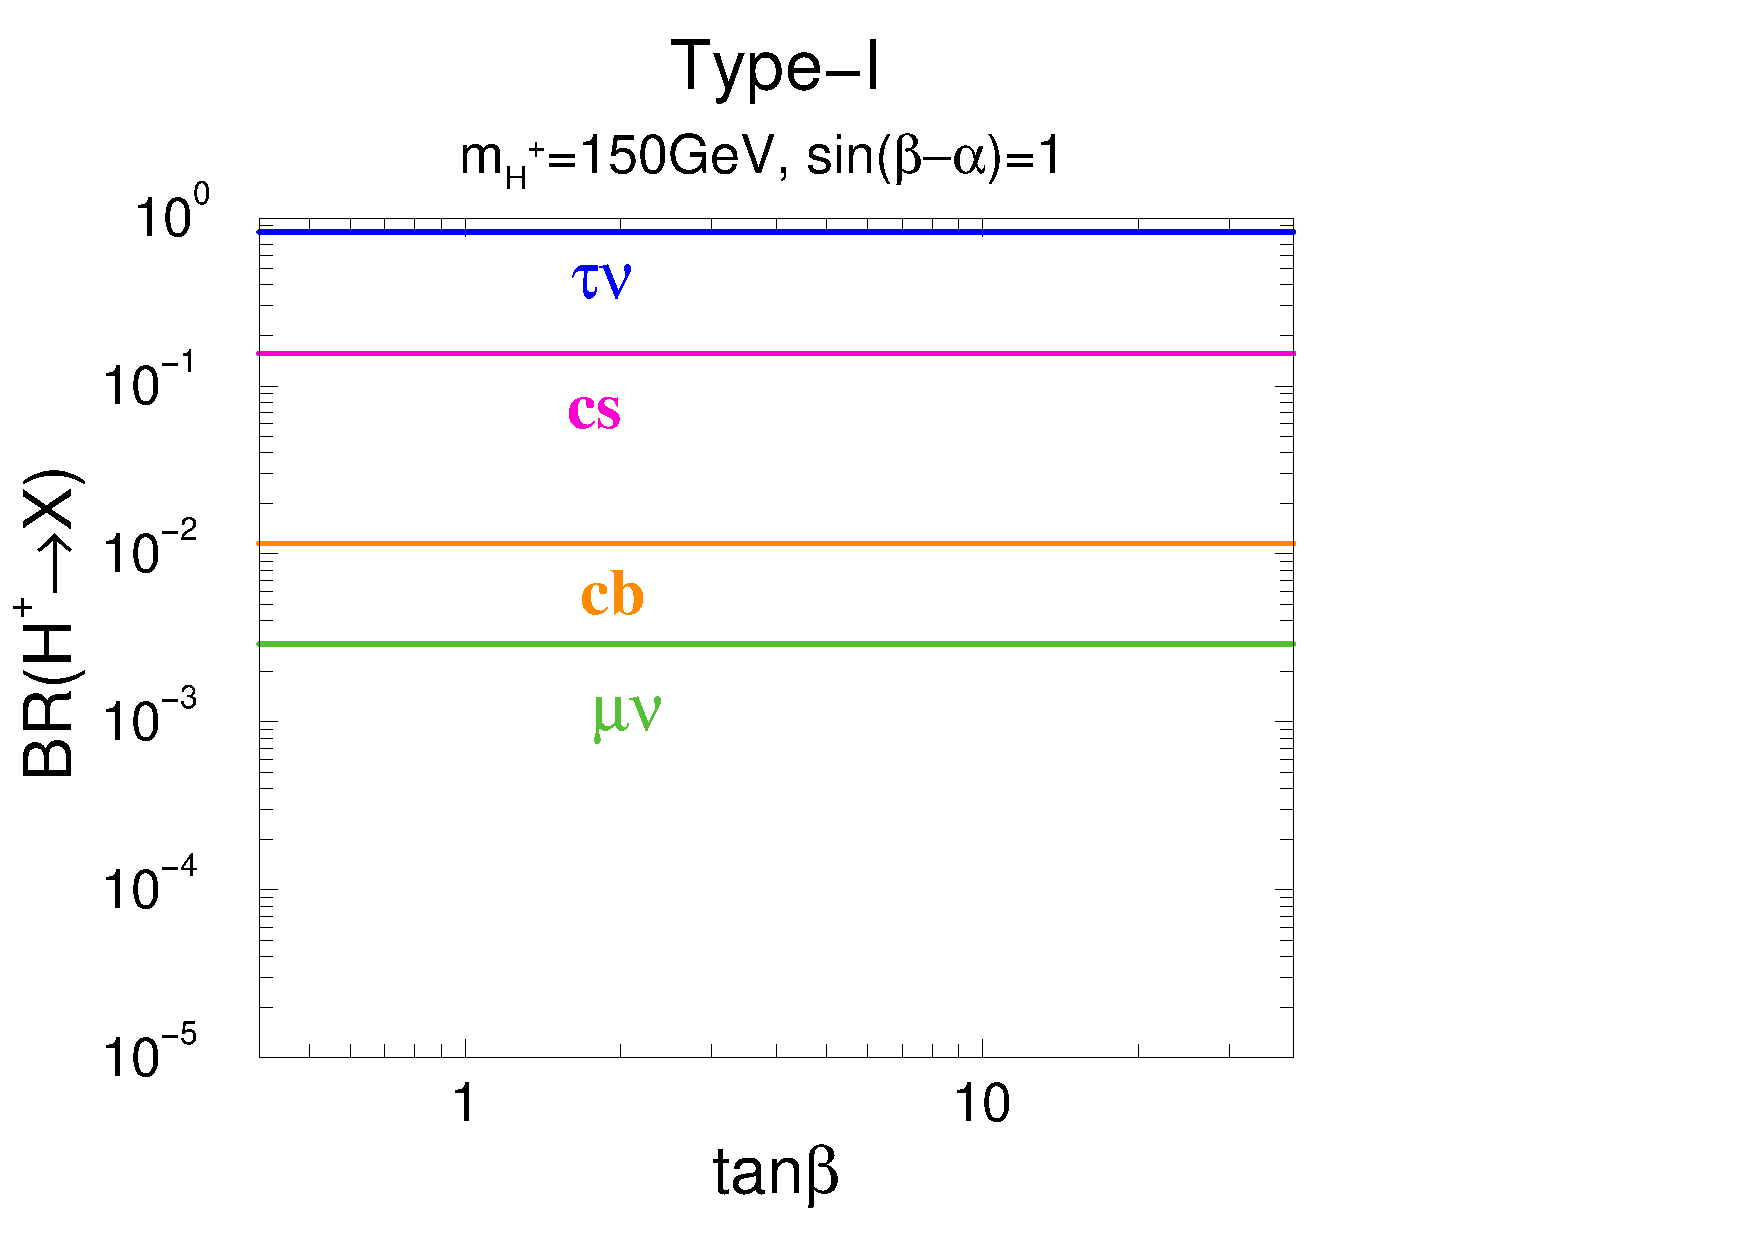
\includegraphics[width=0.49\linewidth]{Theory/Image/BR_ch_1.pdf}}
\subfigure[]{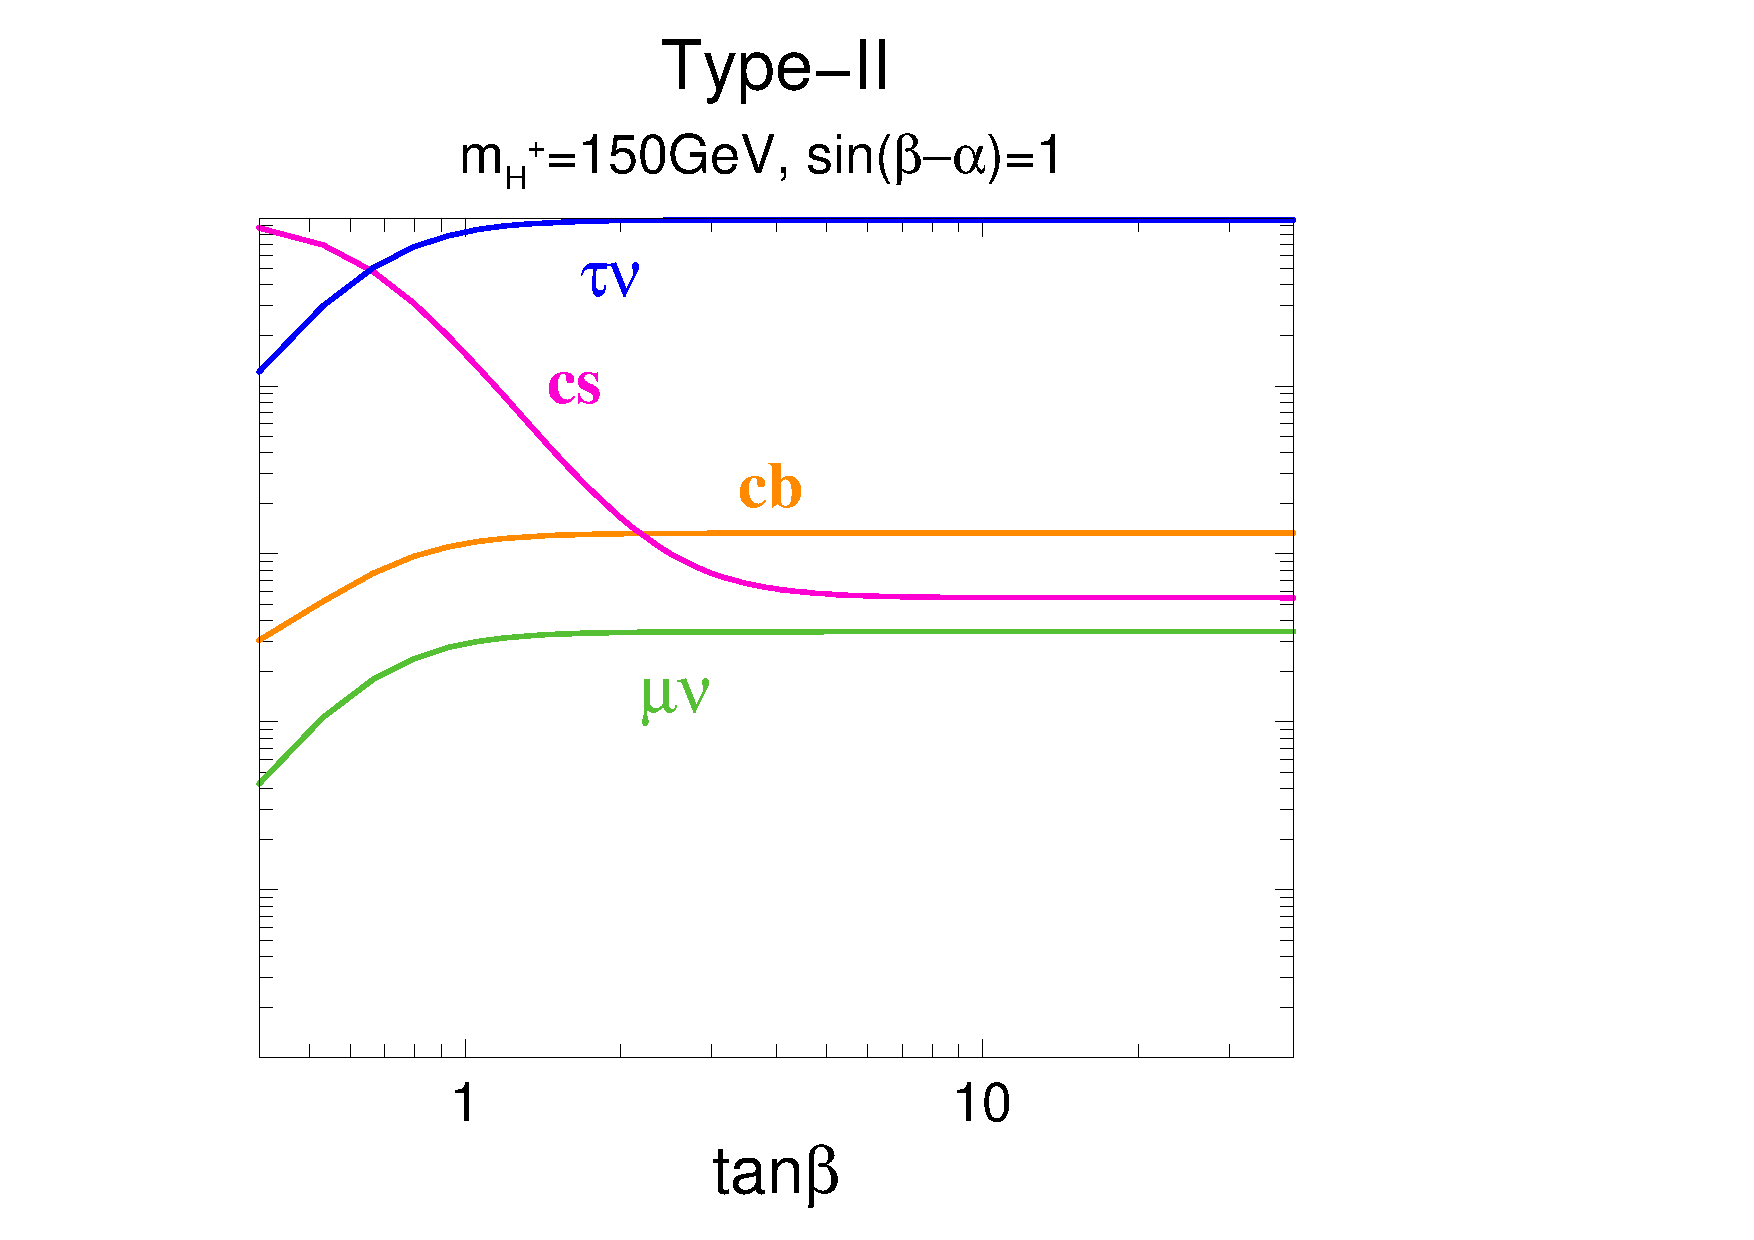
\includegraphics[width=0.49\linewidth]{Theory/Image/BR_ch_2.pdf}}
\vfil
\subfigure[]{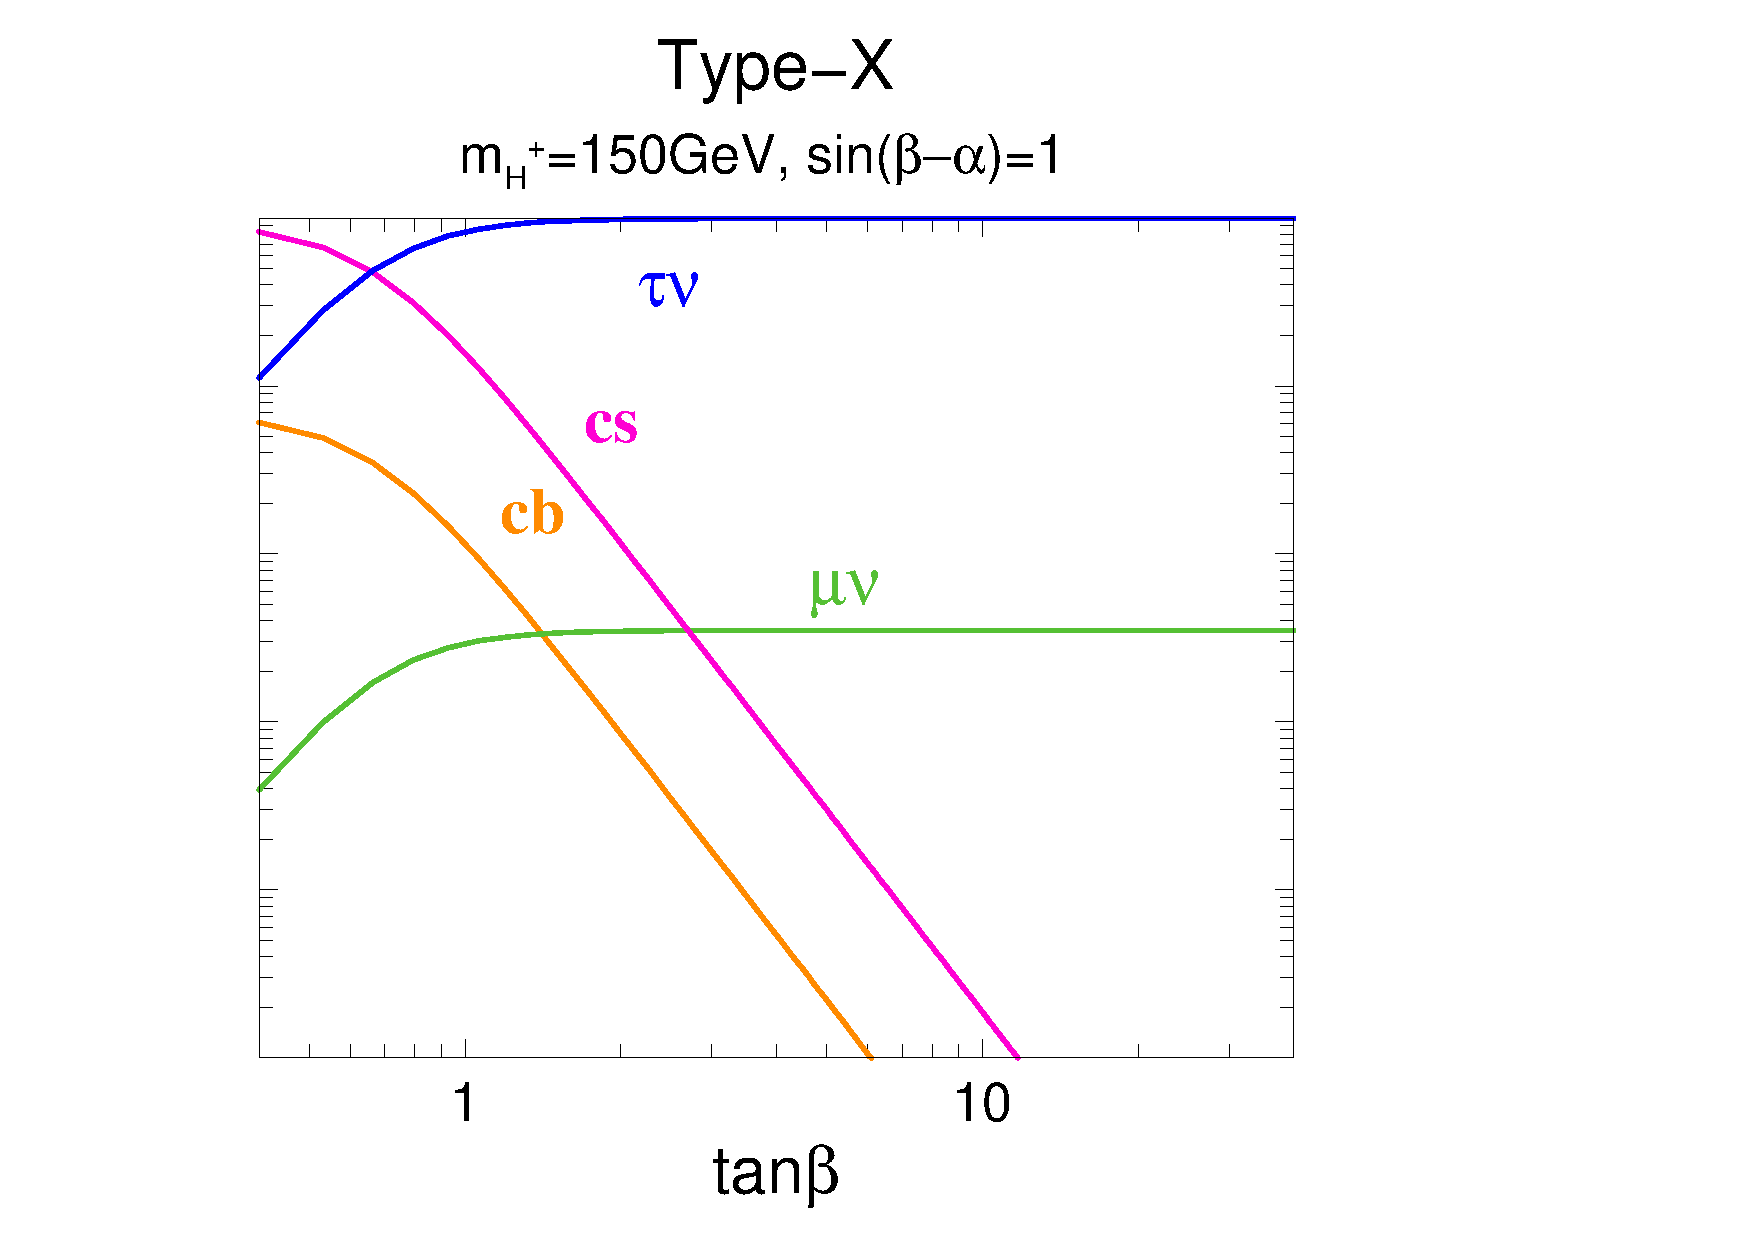
\includegraphics[width=0.49\linewidth]{Theory/Image/BR_ch_X.pdf}}
\subfigure[]{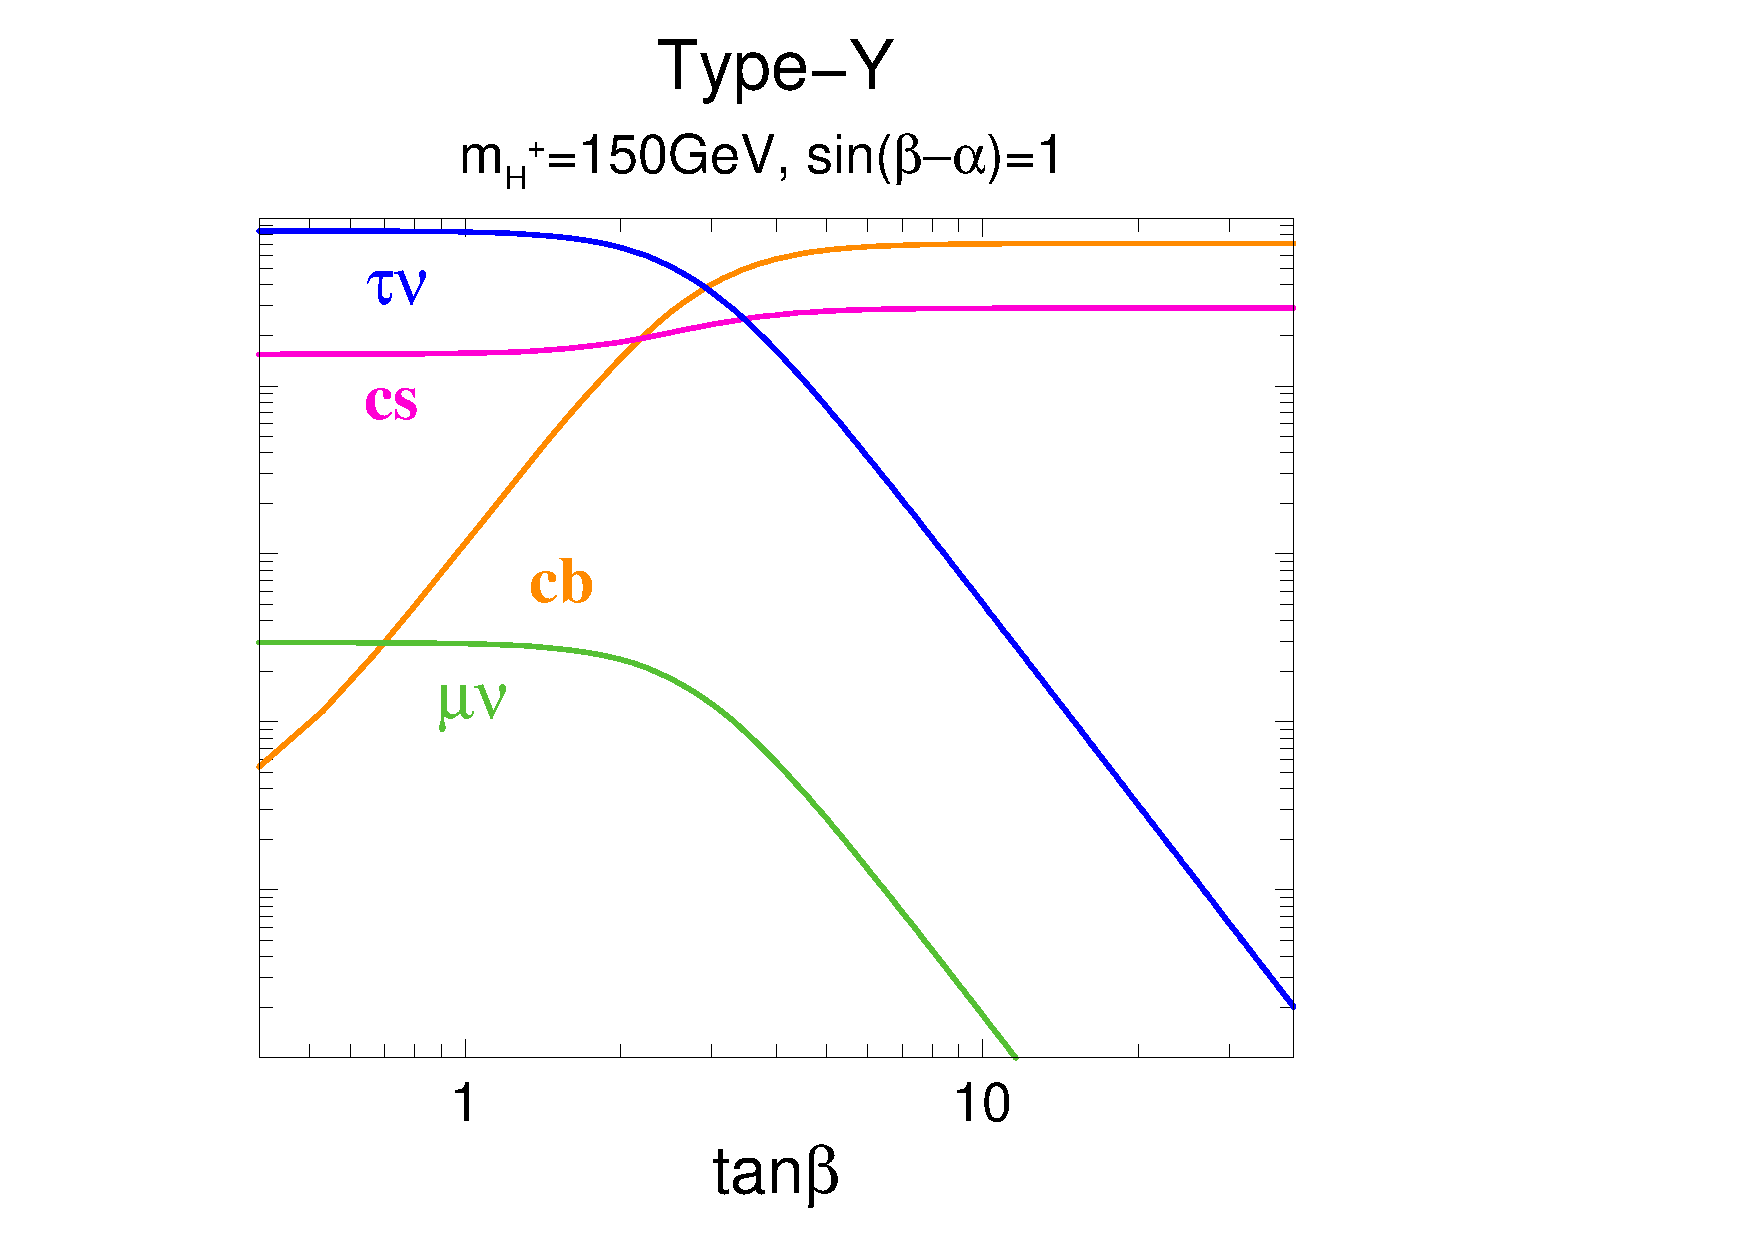
\includegraphics[width=0.49\linewidth]{Theory/Image/BR_ch_Y.pdf}}
\caption{The branching ratio of charged Higgs decay in different channels
	 as a function of $\tan\beta$ for $\mHp$ = 150 \GeV in 
	different types of the 2HDM. These plots are taken from \cite{PhysRevD.80.015017}. }
\label{fig:brHqq}
\end{figure}

